\chapter{Η διεπαφή προγραμματισμού OpenMP}
\label{ch:OpenMP API}

\section{Εισαγωγή στο OpenMP}
\label{sec:Introduction to OpenMP}
Όπως αναφέρθηκε ήδη στην Υποενότητα \ref{ssec:Shared Memory Programming}, η διεπαφή προγραμματισμού εφαρμογών OpenMP (Open Multi-Processing) αναπτύχθηκε για τη διευκόλυνση της ανάπτυξης πολυνηματικών εφαρμογών για συστήματα κοινόχρηστης μνήμης. Οι γλώσσες οι οποίες υποστηρίζονται είναι οι C, C++ και Fortran.
To OpenMP αποτελείται από:
\begin{itemize}
	\item Oδηγίες (directives): Συνιστούν οδηγίες προς τον μεταφραστή για το πώς και τι να εκτελέσει πολυνηματικά. Στις γλώσσες C/C++ χρησιμοποιείται ο μηχανισμός που είναι γνωστός ως pragmas και απευθύνεται στον προεπεξεργαστή. Αυτές οι οδηγίες προστίθενται στο υπάρχον σειριακό πρόγραμμα και μπορούν να αγνοηθούν από έναν μεταφραστή που δεν τις υποστηρίζει. Αυτό είναι μεγάλο προσόν καθώς το ίδιο πρόγραμμα μπορεί να εκτελεστεί σειριακά ή παράλληλα.
	\item Ρουτίνες βιβλιοθήκης: σύνολο συναρτήσεων οι οποίες βοηθούν στη διαχείριση των χαρακτηριστικών των νημάτων και του περιβάλλοντος εκτέλεσης. Για παράδειγμα, η συνάρτηση \texttt{omp\_set\_num\_threads(int)} καθορίζει το πλήθος των νημάτων που θα συμμετάσχουν σε επερχόμενη πολυνηματική εκτέλεση (παράλληλη περιοχή).
	\item Μεταβλητές περιβάλλοντος: χρησιμοποιούνται για τον καθορισμό διάφορων χαρακτηριστικών των νημάτων και του περιβάλλοντος εκτέλεσης. Οι τιμές των μεταβλητών περιβάλλοντος οριστικοποιούνται στην αρχή της εκτέλεσης και χρησιμοποιούνται ως προκαθορισμένες τιμές. Κάποιες από αυτές τις προκαθορισμένες αυτές τιμές μπορούν να τροποποιηθούν σε χρόνο εκτέλεσης με χρήση των διαθέσιμων ρουτινών βιβλιοθήκης.
\end{itemize}

Από τη στιγμή που η παραλληλοποίηση ενός σειριακού προγράμματος μπορεί να γίνει με την απλή προσθήκη οδηγιών στο υπάρχοντα κώδικα, η διαδικασία της παραλληλοποίησης απλοποιείται σε μεγάλο βαθμό και μπορεί να γίνει σταδιακά (π.χ. παραλληλοποίηση ενός βρόγχου for τη φορά) και χωρίς τη χρήση διαφορετικής λογικής, όπως για παράδειγμα θα γινόταν με χρήση των POSIX Threads. 

Ένα από τα σχετικά καινούρια χαρακτηριστικά του OpenMP είναι η δυνατότητα αποστολής κώδικα για εκτέλεση σε συσκευές όπως κάρτες γραφικών γενικού σκοπού (GPGPUs), συνεπεξεργαστές (coprocessors) ή διάφορους άλλους επιταχυντές. Το πλεονέκτημα είναι ότι ο προγραμματιστής δεν χρειάζεται να μάθει να προγραμματίζει σε γλώσσες προγραμματισμού χαμηλού επιπέδου όπως OpenCL, CUDA κλπ για να αξιοποιήσει την επεξεργαστική ισχύ των διαθέσιμων συσκευών. Αυτό το χαρακτηριστικό είναι ιδιαίτερα βοηθητικό σε συστήματα υπολογισμών υψηλών επιδόσεων (High Performance Computing - HPC) όπου υπάρχει η τάση να εξοπλίζεται ένα σύνολο των υπολογιστικών κόμβων με ισχυρούς επιταχυντές για την επίτευξη μεγαλύτερων επιδόσεων. Για παράδειγμα, ο υπερυπολογιστής Aris του Εθνικού Δικτύου Υποδομών και Έρευνας (ΕΔΥΤΕ - GRNET) διαθέτει πλην άλλων:
\begin{itemize}
	\item 18 κόμβους με 2 επεξεργαστές Intel Xeon E5-2660v3 και 2 συνεπεξεργαστές Intel Xeon Phi 7120P.
	\item 44 κόμβους με 2 επεξεργαστές Intel Xeon E5-2660v3 και 2 κάρτες γραφικών NVIDIA K40.
	\item 1 κόμβο με 2 επεξεργαστές Intel E5-2698v4 και 8 κάρτες γραφικών NVIDIA V100 για εκτέλεση προγραμμάτων μηχανικής μάθησης.
\end{itemize}

Λαμβάνοντας υπόψην ότι η διαχείριση των νημάτων μετατίθεται από τον προγραμματιστή στο μεταφραστή, ότι απλοποιούνται ουσιώδη ζητήματα ενός παράλληλου προγράμματος όπως η επίτευξη συγχρονισμού και αμοιβαίου αποκλεισμού, καθώς επίσης ότι μπορούν να αξιοποιηθούν επιταχυντές χωρίς γνώση του πως προγραμματίζονται, γίνεται εύκολα αντιληπτό ότι το OpenMP είναι ένα προσιτό εργαλείο ακόμα και για άτομα χωρίς μεγάλη εμπειρία στον παράλληλο προγραμματισμό. Αυτό το χαρακτηριστικό του OpenMP το κάνει ιδιαίτερα διαδεδομένο σε χρήστες που το υπόβαθρό τους διαφέρει από αυτό της επιστήμης της πληροφορικής, όπως για παράδειγμα φυσικοί, χημικοί, αστρονόμοι κόκ. Ταυτόχρονα όμως, η απόκρυψη των λεπτομερειών χαμηλού επιπέδου είναι πιθανό να καταστήσει σε ορισμένες περιπτώσεις μη εφικτή την εξασφάλιση της μέγιστης αποδοτικότητας του παραλληλισμού.

\section{Το προγραμματιστικό μοντέλο του OpenMP}
Το OpenMP βασίζεται στη χρήση πολλαπλών νημάτων όπως άλλωστε συνηθίζεται στον προγραμματισμό συτημάτων κοινόχρηστης μνήμης καθώς και στο προγραμματιστικό μοντέλο fork-join που συναντάται στις διεργασίες.

Στο μοντέλο fork-join, η εκτέλεση ξεκινάει σειριακά από ένα νήμα (γνωστό ως αρχηγός - master) και σε προκαθορισμένα σημεία όπου απαιτείται παράλληλη εκτέλεση, δημιουργούνται επιπλέον νήματα τα οποία μαζί με το νήμα-αρχηγό συμμετέχουν στον παράλληλο υπολογισμό. Τα σημεία στα οποία πραγματοποιείται παράλληλη εκτέλεση είναι γνωστά ως παράλληλες περιοχές (parallel sections/regions). Μόλις ο παράλληλος υπολογισμός τελειώσει τα νήματα που δημιουργήθηκαν τερματίζουν και η εκτέλεση συνεχίζεται σειριακά από το νήμα-αρχηγό.

Ενδιαφέρον είναι το γεγονός ότι υποστηρίζονται αυθαίρετα πολλές εμφωλευμένες παράλληλες περιοχές, δηλαδή ένα οποιοδήποτε νήμα το οποίο συμμετέχει στην εκτέλεση μιας παράλληλης περιοχής μπορεί να αποτελέσει με τη σειρά του νήμα-αρχηγός και να δημιουργήσει μία νέα παράλληλη περιοχή. Οι εμφωλευμένες παράλληλες περιοχές μπορούν να χρησιμοποιηθούν για την ανάθεση εργασιών με το επιθυμητό μέγεθος κόκκου παραλληλίας (granularity) σε κάθε νήμα.

Είναι χρήσιμο να αναφερθεί πως όταν ξεκινάει να εκτελείται μία διεργασία, χρησιμοποιείται ένα νήμα για την εκτέλεση των εντολών σειριακά και το οποίο νήμα στα πλαίσια του OpenMP ονομάζεται αρχικό νήμα (initial thread).

\section{Εισαγωγή στη διεπαφή προγραμματισμού OpenMP}

Το πλήθος των σελίδων των προδιαγραφών του OpenMP τείνει να αυξάνεται εκθετικά στις τελευταίες εκδόσεις με αποτέλεσμα να είναι αδύνατο να περιγραφούν όλες οι δυνατότητές του στα πλαίσια μίας διπλωματικής εργασίας. Για το λόγο αυτό, θα γίνει περιγραφή ενός υποσυνόλου των διαθέσιμων λειτουργιών, πολλές από τις οποίες αποτελούν τις πιο συνηθισμένες και καλύπτουν τις ανάγκες της πλειοψηφίας των διαθέσιμων εφαρμογών OpenMP. Αυτές οι πιο διαδεδομένες λειτουργίες είναι εικοσιμία (21) στο πλήθος και αποτελούν το λεγόμενο OpenMP Common Core @Ref.

\subsection{Σύνταξη οδηγιών (directives)}
Η γενική μορφή μίας οδηγίας στο OpenMP είναι της μορφής:

\begin{quote}
	\texttt{\textbf{\#pragma omp} \textit{directive-name [[,] clause [[,] clause] ... ] <new-line>}}
\end{quote}

Κάθε οδηγία ξεκινάει υποχρεωτικά με το \texttt{\#pragma omp} και ακολουθεί το όνομά της που καθορίζει ποιά λειτουργία θα εκτελεστεί στην περιοχή του κώδικα που ακολουθεί. Υπάρχουν διάφορες διαθέσιμες οδηγίες οι οποίες μπορούν να χρησιμοποιηθούν, πλην άλλων, για τη δημιουργία παράλληλης ομάδας, το συγχρονισμό των νημάτων και τον ορισμό της πολιτικής με την οποία τα νήματα θα ανατεθούν στους διαθέσιμους επεξεργαστές.

Στη συνέχεια τοποθετούνται προαιρετικά φράσεις (clauses) οι οποίες παραμετροποιούν τις συνθήκες υπό τις οποίες θα εκτελεστεί η λειτουργία που ορίζει η οδηγία. Για παράδειγμα, η φράση \texttt{num\_threads} μπορεί να χρησιμοποιηθεί σε συνδιασμό με την οδηγία δημιουργίας παράλληλης ομάδας για να καθορίσει το επιθυμητό πλήθος των νημάτων που θα συμμετάσχουν στην παράλληλη εκτέλεση. Η σειρά με την οποία αναγράφονται οι φράσεις δεν έχει σημασία.

Το τέλος της οδηγίας σηματοδοτείται από αλλαγή γραμμής (newline).

\subsection{Η οδηγία parallel}
\label{ssec:parallel construct}
Η οδηγία \texttt{parallel} συντάσσεται ως εξής:

\begin{quote}
	\texttt{\textbf{\#pragma omp parallel} \textit{[clause [[,] clause] ... ] <new-line>}} \\
		\texttt{\textit{structured-block}}
\end{quote}

Όταν ένα οποιοδήποτε νήμα συναντήσει μία οδηγία \texttt{parallel}, δημιουργείται μία ομάδα νημάτων η οποία εκτελεί την παράλληλη περιοχή. Μια παράλληλη περιοχή υποδηλώνει ένα τμήμα κώδικα το οποίο προορίζεται για πολυνηματική εκτέλεση. Στη συγκεκριμένη περίπτωση, ο κώδικας που περιέχεται στο δομημένο τμήμα κώδικα (structured block) που ακολουθεί την οδηγία \texttt{parallel} είναι αυτός που εν τέλει θα εκτελεστεί παράλληλα. Ώς δομημένο τμήμα κώδικα ορίζεται μία εντολή ή μία ακολουθία εντολών που περικλείονται από άγκιστρα.

Το πλήθος των νημάτων ($N$) που συμμετέχουν σε μια παράλληλη ομάδα είναι σταθερό καθόλη τη διάρκειά της. Το νήμα το οποίο συνάντησε την οδηγία \texttt{parallel} λαμβάνει το ρόλο του αρχηγού (master\footnote{Στο πρότυπο του OpenMP 5.1 (Νοέμβριος 2020) καθορίζεται αλλαγή της ονομασίας master σε primary. Στο παρόν κείμενο θα ακολουθηθεί η ορολογία master (αρχηγός) για λόγους συμβατότητας με τους υπάρχοντες πόρους της Ομάδας Παράλληλης Επεξεργασίας του Πανεπιστημίου Ιωαννίνων.}) της ομάδας, ενώ συμμετέχει και αυτό στον παράλληλο υπολογισμό μαζί με τα υπόλοιπα $N-1$ νήματα που δημιουργήθηκαν.

Μέσα σε μία παράλληλη περιοχή μπορούν να χρησιμοποιηθούν τα αναγνωριστικά των νημάτων για την αναγνώριση του κάθε νήματος. Τα αναγνωριστικά είναι ακέραιοι αριθμοί και συγκεκριμένα για μία ομάδα $N$ νημάτων, η τιμή τους κυμαίνεται από μηδέν (για τον αρχηγό της ομάδας) έως και ένα λιγότερο από το μέγεθος της ομάδας, δηλαδή $N-1$.

Καθώς ο χρόνος που χρειάζεται ένα νήμα για να εκτελέσει την παράλληλη περιοχή εξαρτάται από πολλούς παράγοντες, όπως για παράδειγμα το πόσο δίκαιη είναι η κατανομή του φόρτου μεταξύ των νημάτων της ομάδας, στο τέλος της παράλληλης περιοχής υπονοείται μία κλήση φραγής (barrier). Η κλήση αυτή εξασφαλίζει ότι τα νήματα θα περιμένουν στην κλήση φραγής μέχρις ότου όλα τα νήματα να φτάσουν σε αυτό το σημείο πριν τους επιτραπεί να τερματίσουν και το νήμα-αρχηγός συνεχίσει την εκτέλεση του υπόλοιπου προγράμματος που ακολουθεί της παράλληλης περιοχής.

Την οδηγία \texttt{parallel} μπορεί προεραιτικά να ακολουθούν φράσεις διαμοιρασμού δεδομένων που θα δούμε στην Υποενότητα \ref{ssec:Data sharing clauses} καθώς και οι φράσεις \texttt{num\_threads}, \texttt{redution} και \texttt{proc\_bind} που περιγράφονται αμέσως μετά.

\subsubsection{Η φράση num\_threads}
Η φράση \texttt{num\_threads} δέχεται ως παράμετρο έναν ακέραιο αριθμό και καθορίζει το επιθυμητό πλήθος των νημάτων που θα εκτελέσουν την παράλληλη περιοχή.

\subsubsection{Η φράση reduction}
Η φράση \texttt{reduction} χρησιμοποιείται για τη διεκπεραίωση μιας αριθμητικής πράξης από τα νήματα της ομάδας πάνω σε μια κοινόχρηστη μεταβλητή, εξασφαλίζοντας την αποφυγή συνθηκών ανταγωνισμού. Η απλουστευμένη σύνταξη της φράσης είναι η εξής:
\begin{quote}
	\texttt{\textbf{reduction(}\textit{reduction-identifier : list}\textbf{)}}
\end{quote}

Ο \texttt{reduction-identifier} είναι η πράξη η οποία θέλουμε να εφαρμοστεί πάνω στις μία ή περισσότερες μεταβλητές που αναγράφονται στη λίστα \texttt{list} και είναι διαχωρισμένες μεταξύ τους με κόμμα. Οι διαθέσιμες πράξεις είναι οι \texttt{+}, \texttt{-}, \texttt{*}, \texttt{\&}, \texttt{\textbar}, \texttt{\string^}, \texttt{\&\&} και \texttt{\textbar\textbar}.

\subsubsection{Η φράση proc\_bind}
Η φράση \texttt{proc\_bind} χρησιμοποιείται για τον ορισμό της πολιτικής με την οποία τα νήματα θα ανατεθούν στους διαθέσιμους επεξεργαστές. Οι διαθέσιμες επιλογές είναι οι \texttt{master/primary}, \texttt{close} και \texttt{spread}. Περισσότερες λεπτομέρειες θα δούμε στην Υποενότητα \ref{sec:Topology in OpenMP} όπου θα ασχοληθούμε λεπτομερώς με την τοπολογία του υποκείμενου συστήματος και τον τρόπο ανάθεσης των νημάτων OpenMP στους επεξεργαστές.


\subsection{Φράσεις διαμοιρασμού δεδομένων}
\label{ssec:Data sharing clauses}
Οι φράσεις διαμοιρασμού δεδομένων χρησιμοποιούνται για να δηλώσουν τον τρόπο διαμοιρασμού μίας ή περισσότερων μεταβλητών μεταξύ των νημάτων ως εξής:
\begin{itemize}
	\item \texttt{shared}: Οι μεταβλητές είναι κοινόχρηστες.
	\item \texttt{private}: Οι μεταβλητές είναι ιδιωτικές καθώς δημιουργείται από ένα αντίγραφο για κάθε νήμα.
	\item \texttt{firstprivate}: Οι μεταβλητές είναι ιδιωτικές και καθεμιά αρχικοποιείται στην τιμή της αντίστοιχης αρχικής μεταβλητής.
	\item \texttt{lastprivate}: Οι μεταβλητές είναι ιδιωτικές και μετά το πέρας της εκτέλεσης η τιμή της καθεμιάς τους θα χρησιμοποιηθεί για την ενημέρωση της τιμής της αντίστοιχης αρχικής μεταβλητής.
	\item \texttt{default}: Καθορίζει την προκαθορισμένη πολιτική διαμοιρασμού με διαθέσιμες επιλογές να είναι οι \texttt{shared}, \texttt{firstprivate}, \texttt{private}, \texttt{none}.
\end{itemize}


\subsection{Οδηγίες Διαμοιρασμού Εργασίας}
\label{ssec:Work sharing directives}
Το OpenMP παρέχει τη δυνατότητα κατανομής του φόρτου εργασίας ανάμεσα στα νήματα της ομάδας μέσω των οδηγιών που καθορίζουν περιοχές διαμοιρασμού εργασίας (worksharing regions).

Η βασική διαφορά μίας περιοχής διαμοιρασμού εργασίας με μία παράλληλη περιοχή είναι ότι στην πρώτη σε αντίθεση με τη δεύτερη, δεν δημιουργούνται νέα νήματα αλλά χρησιμοποιούνται τα υπάρχοντα. Βάσει αυτής της παρατήρησης συμπεραίνουμε ότι οι περιοχές διαμοιρασμού έχουν νόημα όταν εντοπίζονται εντός παράλληλων περιοχών. Είναι πιθανό μία παράλληλη ομάδα που αποτελείται από ένα μόνο νήμα να συναντήσει μία οδηγία περιοχής διαμοιρασμού εργασίας. Όπως είναι προφανές, σε αυτή την περίπτωση, η εκτέλεση είναι σειριακή και όχι παράλληλη.

Στο τέλος των περιοχών διαμοιρασμού εργασίας, όπως και στο τέλος των παράλληλων περιοχών, υπονοείται μία κλήση φραγής για την επίτευξη συγχρονισμού μεταξύ των νημάτων, με τη διαφορά ότι στις πρώτες η κλήση φραγής μπορεί να παραληφθεί με τη χρήση της φράσης \texttt{nowait}.

\subsubsection{Οδηγία sections}
Χρησιμοποιείται για την κατανομή μη επαναληπτικών (non-iterative) εργασιών και συντάσσεται ως εξής:
\begin{quote}
	\texttt{\textbf{\#pragma omp sections} \textit{[clause [[,] clause] ... ] <new-line>}} \\
	\texttt{\{} \\
		\texttt{\textit{[} \textbf{\#pragma omp section} \textit{<new-line>}} \\
		\texttt{\textit{<structured-block> ]}} \\
		\texttt{\textit{[} \textbf{\#pragma omp section} \textit{<new-line>}} \\
		\texttt{\textit{<structured-block> ]}} \\
		... \\
	\texttt{\}}
\end{quote}

Κάθε δομημένο τμήμα κώδικα που ακολουθεί μία οδηγία \texttt{\#pragma omp section} που περιέχεται μέσα στην οδηγία \texttt{sections} θα ανατεθεί σε ένα νήμα και θα εκτελεστεί ακριβώς μία φορά. Συνήθεις φράσεις αποτελούν οι \texttt{private}, \texttt{firstprivate}, \texttt{lastprivate} και \texttt{reduction}.

\subsubsection{Οδηγία single}
Η οδηγία αυτή καθορίζει ότι το δομημένο τμήμα κώδικα που την ακολουθεί θα εκτελεστεί μόνο από ένα νήμα (όχι απαραίτητα το νήμα-αρχηγό) και η σύνταξή της είναι η εξής:
\begin{quote}
	\texttt{\textbf{\#pragma omp single} \textit{[clause [[,] clause] ... ] <new-line>}} \\
		\texttt{\textit{<structured-block>}}
\end{quote}

Συνήθεις φράσεις που ακολουθούν είναι οι \texttt{private} και \texttt{firstprivate}.


\subsection{Οδηγίες Διαμοιρασμού Εργασίας Βρόγχου}
Οι οδηγίες διαμοιαρμού εργασίας βρόγχου είναι αντίστοιχες με τις οδηγίες διαμοιρασμού εργασίας που είδαμε στην Υποενότητα \ref{ssec:Work sharing directives}, με τη διαφορά ότι αφορούν την κατανομή των επαναλήψεων ενός βρόγχου στα νήματα.

\subsubsection{Οδηγία for}
Χρησιμοποιείται για την κατανομή των επαναλήψεων ενός βρόγχου\footnote{Η σύνταξη του βρόγχου δεν μπορεί να είναι τόσο αυθαίρετη όσο επιτρέπει το συντακτικό των γλωσσών C/C++, αλλά στα πλαίσια αυτής της εργασίας δεν θα μας απασχολήσει αυτό το ζήτημα.} \texttt{for} και συντάσσεται ως εξής:
\begin{quote}
	\texttt{\textbf{\#pragma omp for} \textit{[clause [[,] clause] ... ] <new-line>}} \\
		\texttt{\textit{<loop-nest>}}
\end{quote}

Την οδηγία αυτή ακολουθεί υποχρεωτικά βρόγχος \texttt{for} ενώ συνήθεις φράσεις αποτελούν οι \texttt{private}, \texttt{firstprivate}, \texttt{lastprivate}, \texttt{reduction} και \texttt{schedule}.

Η φράση \texttt{schedule} χρησιμοποιείται για τον καθορισμό της πολιτικής με την οποία θα διαμοιραστούν οι επαναλήψεις ενός βρόγχου \texttt{for} στα νήματα και η απλουστευμένη σύνταξη της είναι η ακόλουθη:
\begin{quote}
	\texttt{\textbf{schedule(}\textit{kind[, chunk\_size]}\textbf{)}}
\end{quote}

Η τιμή \texttt{kind} καθορίζει τον τρόπο διαμοιρασμού των επαναλήψεων ενώ η τιμή \texttt{chunk\_size} καθορίζει το μέγεθος του κόκκου παραλληλίας (granularity) που αναλαμβάνει το κάθε νήμα. Η χρονοδρομολόγηση των επαναλήψεων γίνεται όπως περιγράφεται ακολούθως:
\begin{itemize}
	\item \texttt{static}: Συνεχόμενες επαναλήψεις διασπώνται σε τμήματα μεγέθους όσο η τιμή \texttt{chunk\_size} και ανατίθενται κυκλικά (round-robin) στα νήματα βάσει του αναγνωριστικού τους. Σε περίπτωση που δεν έχει καθοριστεί συγκεκριμένη τιμή \texttt{chunk\_size}, το σύνολο των επαναλήψεων χωρίζεται σε τόσα ισομεγέθη τμήματα όσα και το πλήθος των νημάτων.
	\item \texttt{dynamic}: Συνεχόμενες επαναλήψεις διασπώνται σε τμήματα μεγέθους όσο η τιμή \texttt{chunk\_size} και ανατίθενται στα νήματα όταν αυτά ζητήσουν το επόμενο τμήμα προς εκτέλεση. Η δυναμική ανάθεση συνεχίζεται μέχρι να ανατεθούν όλα τα τμήματα. Σε περίπτωση που δεν έχει καθοριστεί συγκεκριμένη τιμή \texttt{chunk\_size}, τότε τα τμήματα έχουν μέγεθος ίσο με 1.
	\item \texttt{guided}: Η πολιτική αυτή μοιάζει στην πολιτική \texttt{dynamic} με τη διαφορά ότι το μέγεθος των τμημάτων δεν είναι σταθερό. Συγκεκριμένα, για \texttt{chunk\_size} ίσο με 1 ($k$), το μέγεθος του πρώτου τμήματος ισούται με το πλήθος όλων των επαναλήψεων διαιρεμένο με το πλήθος των νημάτων, με το μέγεθος των επόμενων τμημάτων να μειώνεται εκθετικά μέχρι να ισούται με 1 ($k$).
	\item \texttt{auto}: Η επιλογή πολιτικής και μεγέθους κόκκου παραλληλίας μεταφέρεται από τον προγραμματιστή στο μεταφραστή ή στο σύστημα χρόνου εκτέλεσης (runtime).
	\item \texttt{runtime}: Η πολιτική και το μέγεθος κόκκου παραλληλίας καθορίζονται σε χρόνο εκτέλεσης βάσει της τιμής της μεταβλητής περιβάλλοντος \texttt{OMP\_SCHEDULE}.
\end{itemize}

Στην περίπτωση των πολιτικών \texttt{auto} και \texttt{runtime} απαγορεύεται ο προσδιορισμός τιμής \texttt{chunk\_size}.

\subsection{Η οδηγία task}
Η οδηγία αυτή ορίζει μία εργασία προς εκτέλεση και συντάσσεται ως εξής:
\begin{quote}
	\texttt{\textbf{\#pragma omp task} \textit{[clause [[,] clause] ... ] <new-line>}} \\
		\texttt{\textit{<structured-block>}}
\end{quote}

Όταν ένα νήμα συναντήσει την οδηγία \texttt{task}, δημιουργεί μία νέα εργασία που αποτελείται από τον κώδικα του δομημένου τμήματος κώδικα και το περιβάλλον δεδομένων (data environment) που χρειάζεται η εργασία για να διεκπεραιωθεί. Η εκτέλεση της εργασίας μπορεί να πραγματοποιηθεί από οποιοδήποτε νήμα και δεν είναι γνωστό πότε θα ξεκινήσει. Να σημειωθεί ότι υποστηρίζονται εμφωλευμένες οδηγίες \texttt{task}.

Συνήθεις φράσεις αποτελούν οι \texttt{default}, \texttt{private}, \texttt{firstprivate} και \texttt{shared}.


\subsection{Οδηγίες συγχρονισμού}
Στα προγράμματα OpenMP ως προγράμματα για συστήματα κοινόχρηστης μνήμης, σημαντικός είναι ο ρόλος του συγχρονισμού για την εξασφάλιση της συνέπειας των δεδομένων και της ορθότητας του προγράμματος. Για το λόγο αυτό, το OpenMP παρέχει έτοιμες λειτουργίες συγχρονισμού ως οδηγίες.

\subsubsection{Οδηγία atomic}
Απλουστευμένη σύνταξη:
\begin{quote}
	\texttt{\textbf{\#pragma omp atomic} \textit{<new-line>}} \\
		\texttt{\textit{<statement>}}
\end{quote}

Εξασφαλίζει ότι μια θέση μνήμης προσβαίνεται ατομικά εξαλείφοντας την πιθανότητα πολλαπλών ταυτόχρονων προσβάσεων από διαφορετικά νήματα.

\subsubsection{Οδηγία barrier}
Σύνταξη:
\begin{quote}
	\texttt{\textbf{\#pragma omp barrier} \textit{<new-line>}}
\end{quote}

Η γνωστή κλήση φραγής η οποία εξασφαλίζει ότι όλα τα νήματα της ομάδας θα περιμένουν σε αυτό το σημείο πριν μπορέσουν να συνεχίσουν την εκτέλεση με τις εντολές που ακολουθούν.

\subsubsection{Οδηγία critical}
Απλουστευμένη σύνταξη:
\begin{quote}
	\texttt{\textbf{\#pragma omp critical} \textit{<new-line>}} \\
		\texttt{\textit{<structured-block>}}
\end{quote}

Εξασφαλίζει ότι το δομημένο τμήμα κώδικα που ακολουθεί θα εκτελείται από ένα νήμα μόνο τη φορά.

\subsubsection{Οδηγία taskwait}
Απλουστευμένη σύνταξη:
\begin{quote}
	\texttt{\textbf{\#pragma omp taskwait} \textit{<new-line>}}
\end{quote}

Εξασφαλίζει ότι οι εργασίες-παιδιά της τρέχουσας εργασίας (task) θα έχουν ολοκληρωθεί πριν συνεχιστεί η εκτέλεση μετά από αυτό το σημείο.

\subsection{Ρουτίνες βιβλιοθήκης χρόνου εκτέλεσης}
\begin{itemize}
	\item \texttt{void omp\_set\_num\_threads(int num\_threads)}: Θέτει την τιμή της παραμέτρου \texttt{num\_threads} ως το πλήθος των νημάτων που θα χρησιμοποιηθούν σε επερχόμενες παράλληλες περιοχές. Εξαίρεση αποτελούν οι παράλληλες περιοχές που χρησιμοποιούν τη φράση \texttt{num\_threads} η οποία υπερισχύει.
	\item \texttt{int omp\_get\_num\_threads(void)}: Επιστρέφει το πλήθος των νημάτων που συνιστούν την τρέχουσα ομάδα.
	\item \texttt{int omp\_get\_thread\_num(void)}: Επιστρέφει το αριθμητικό αναγνωριστικό του καλούντος νήματος μέσα στο πλαίσιο της τρέχουσας ομάδας.
	\item \texttt{double omp\_get\_wtime(void)}: Επιστρέφει το χρόνο (wall clock) σε δευτερόλεπτα που παρήλθε μετά από μία δεδομένη αλλά ταυτόχρονα αυθαίρετη στιγμή στο παρελθόν.
\end{itemize}

\subsection{Μεταβλητές περιβάλλοντος}
Η μεταβλητή περιβάλλοντος \texttt{OMP\_NUM\_THREADS} μπορεί να χρησιμοποιηθεί για τον ορισμό ενός προκαθορισμένου πλήθους νημάτων που θα συμμετέχουν στις παράλληλες περιοχές του προγράμματος. Η τελική απόφαση για το πλήθος των νημάτων που θα χρησιμοποιηθούν σε μία παράλληλη περιοχή καθορίζεται σε φθίνουσα προτεραιότητα από:
\begin{enumerate}
	\item Τη μεταβλητή περιβάλλοντος \texttt{OMP\_NUM\_THREADS}
	\item Τη ρουτίνα βιβλιοθήκης χρόνου εκτέλεσης \texttt{omp\_set\_num\_threads}
	\item Τη φράση \texttt{num\_threads} της οδηγίας \texttt{parallel}
\end{enumerate}


\section{Μεταφραστές OpenMP}
Η διεπαφή που ορίζεται από το πρότυπο του OpenMP υλοποιείται από διάφορους εμπορικούς και ερευνητικούς μεταφραστές. Προμηθευτές μεταφραστών για C/C++ που υποστηρίζουν το OpenMP είναι οι εξής:

\begin{itemize}
	\item AMD: 
	\begin{itemize}
		\item Ο AOMP είναι βασισμένος στον LLVM/Clang και υποστηρίζει την εκτέλεση κώδικα σε πολλαπλές κάρτες γραφικών/επιταχυντές.
		\item Ο AOCC είναι επίσης βασισμένος στον clang/LLVM και υποστηρίζει πλήρως το OpenMP 4.5 και μερικώς το OpenMP 5.0.
	\end{itemize}
	\item ARM: Ο μεταφραστής της ARM παρέχει πλήρη υποστήριξη για το OpenMP 3.1 και υποστηρίζει το OpenMP 4.0/4.5 χωρίς τη δυνατότητα εκτέλεσης κώδικα σε συσκευές η οποία βρίσκεται υπό ανάπτυξη.
	\item Barcelona Supercomputing Center: Ο Mercurium είναι ένας ερευνητικός μεταφραστής πηγαίου σε πηγαίο κώδικα (source-to-source) ο οποίος υποστηρίζει σχεδόν πλήρως το OpenMP 3.1 καθώς και χαρακτηριστικά νεότερων εκδόσεων που σχετίζονται με τον μηχανισμό tasking του OpenMP.
	\item Fujitsu: Οι μεταφραστές για τον υπερυπολογιστή PRIMEHPC FX100 της Fujitsu υποστηρίζουν το OpenMP 3.1.
	\item GNU: Ο GCC υποστηρίζει πλήρως το OpenMP 4.5 (έκδοση 6) και μερικώς το OpenMP 5.0. Επίσης, σε συστήματα Linux υποστηρίζει την εκτέλεση κώδικα σε κάρτες γραφικών NVIDIA (nvptx) και τις κάρτες Fiji και Vega της AMD Radeon (GCN).
	\item HPE: Το Cray Compiling Environment (CCE) παρέχει πλήρη υποστήριξη για το OpenMP 4.5 και μερική υποστήριξη για το OpenMP 5.0.
	\item IBM: Ο μεταφραστής XL C/C++ για Linux υποστηρίζει πλήρως το OpenMP 4.5.
	\item Intel: Οι μεταφραστές της Intel υποστηρίζουν πλήρως το OpenMP 4.5 και μερικώς το OpenMP 5.0.
	\item LLNL Rose Research Compiler: Ο ROSE είναι ένας ερευνητικός μετφραστής πηγαίου σε πηγαίο κώδικα που υποστηρίζει το OpenMP 3.0 και κάποια χαρακτηριστικά του OpenMP 4.0 που σχετίζονται με την εκτέλεση κώδικα σε κάρτες γραφικών/επιταχυντές της NVIDIA.
	\item LLVM: Ο Clang παρέχει υποστήριξη για το OpenMP 4.5 με περιορισμένη υποστήριξη για την εκτέλεση κώδικα σε συσκευές. Επίσης, υποστηρίζεται μεγάλο μέρος του OpenMP 5.0 και μικρό μέρος του OpenMP 5.1.
	\item Siemens: Ο Sourcery CodeBench (AMD GCN) Lite για συστήματα x86\_64 GNU/Linux είναι βασισμένος στον GCC, παρέχει πλήρη υποστήριξη για το OpenMP 4.5, μερική υποστήριξη για το OpenMP 5.0. και επιτρέπει την εκτέλεση κώδικα σε κάρτες γραφικών AMD Radeon (GCN) όπως οι Fiji, gfx900 Vega 10 και gfx906 Vega 20.	
	\item NVIDIA HPC Compiler: Οι μεταφραστές NVIDIA HPC παρέχουν πλήρη υποστήριξη του OpenMP 3.1 και μερική υποστήριξη του OpenMP 5.0 για συστήματα Linux/x86-64, Linux/OpenPOWER, Linux/Arm. Επίσης, σε κάρτες γραφικών της NVIDIA υποστηρίζεται μερικώς το OpenMP 5.0.
	\item OpenUH Research Compiler: Ο OpenUH είναι ερευνητικός μεταφραστής και υποστηρίζει πλήρως το OpenMP 2.5 και σχεδόν πλήρως το OpenMP 3.0 σε συστήματα Linux.
	\item Oracle: Οι μεταφραστές του Oracle Developer Studio υποστηρίζουν το OpenMP 4.0.
	\item PGI: Οι μεταφραστές NVidia HPC υποστηρίζουν μερικώς το OpenMP 5.0.
	\item Texas Instruments:
		\begin{itemize}
			\item Ο μεταφραστής TI cl6x υποστηρίζει το OpenMP 3.0. (C66x).
			\item Το βασισμένο στον GCC Linaro toolchain υποστηρίζει το OpenMP 4.5 (Cortex-A15).
			\item Ο μεταφραστής TI clacc υποστηρίζει το OpenMP 3.0 και εκτέλεση κώδικα σε συσκευές βάσει του OpenMP 4.0 (Cortex-A15+C66x-DSP).
		\end{itemize}
		Να σημειωθεί ότι η παρεχόμενη υποτήριξη αφορά προϊόντα system on a chip (SoC) της Texas Instruments.
\end{itemize}


\subsection{Ο μεταφραστής OMPi}
Ο μεταφραστής OMPi αναπτύσσεται από την Ομάδα Παράλληλης Επεξεργασίας του Πανεπιστημίου Ιωαννίνων από το 2001 και είναι ένας μεταφραστής για τη γλώσσα C που υποστηρίζει τη διεπαφή προγραμματισμού εφαρμογών OpenMP. Ο OMPi είναι οργανωμένος σε δύο βασικά μέρη, τον μεταφραστή (compiler) και το σύστημα χρόνου εκτέλεσης (runtime).

% Το τμήμα του μεταφραστή δέχεται ως είσοδο προγράμματα πηγαίου κώδικα σε γλώσσα C που περιλαμβάνουν οδηγίες OpenMP και ως έξοδο παράγει προγράμματα στα οποία οι οδηγίες αυτές έχουν αντικατασταθεί από κλήσεις συναρτήσεων του συστήματος χρόνου εκτέλεσης και οι οποίες υλοποιούν τις λειτουργίες που καθορίζουν οι αντίστοιχες οδηγίες OpenMP. Ο παραγόμενος πηγαίος κώδικας είναι έτοιμος προς μετάφραση από έναν μεταφραστή γλώσσας C (π.χ. GCC) που είναι εγκατεστημένος στο σύστημα ώστε να παραχθεί εν τέλει το εκτελέσιμο αρχείο.

\subsubsection{Διαδικασία μετάφρασης προγραμμάτων χρήστη}
Η πλήρης διαδικασία μετάφρασης που ακολουθεί ο OMPi φαίνεται στο Σχήμα \ref{fig:ompi-translation}. Το πρόγραμμα εισόδου είναι πηγαίος κώδικας σε γλώσσα C που περιλαμβάνει οδηγίες OpenMP. Όπως συμβαίνει με όλα τα προγράμματα C, αρχικά περνάνε από το στάδιο της προεπεξεργασίας. Η έξοδος αυτού του πρώτου σταδίου τροφοδοτείται στο τμήμα του μεταφραστή (compiler) του OMPi, ο οποίος κάνει λεκτική και συντακτική ανάλυση. Από τη συντακτική ανάλυση προκύπτει το αφηρημένο συντακτικό δέντρο (AST - Abstract Syntax Tree) το οποίο χρησιμεύει στην αντικατάσταση των οδηγιών OpenMP με κλήσεις συναρτήσεων του συστήματος χρόνου εκτέλεσης, οι οποίες υλοποιούν τις λειτουργίες που καθορίζουν οι αντίστοιχες οδηγίες. Στη συνέχεια, ο μετασχηματισμένος κώδικας δίνεται ως είσοδος σε έναν απλό μεταφραστή για γλώσσα C (π.χ. GCC) ώστε να παραχθεί το αντικείμενο πρόγραμμα. Τέλος, από τη σύνδεση (linking) του αντικείμενου προγράμματος με τη βιβλιοθήκη χρόνου εκτέλεσης του OMPi και τις βιβλιοθήκες του συστήματος, προκύπτει το τελικό εκτελέσιμο αρχείο.

\begin{figure}[t]
	\centering
	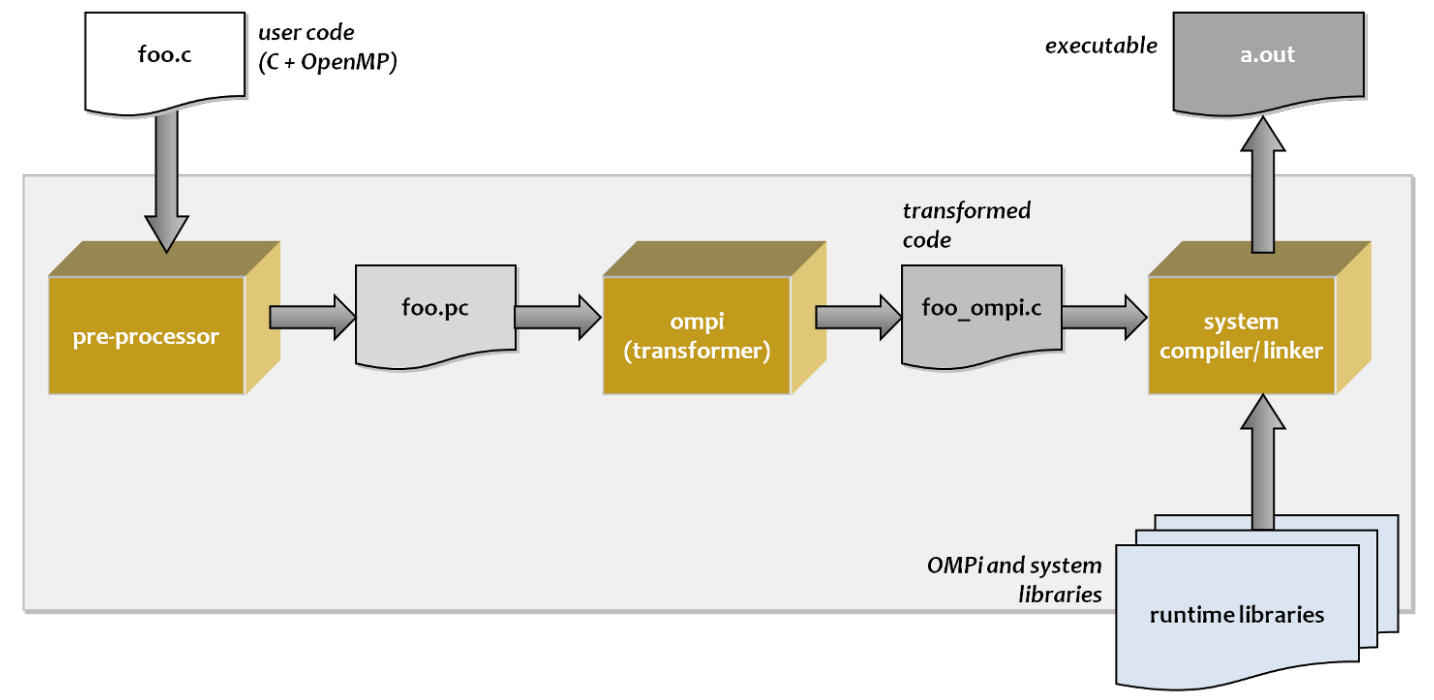
\includegraphics[width=0.9\textwidth]{Figures/ompi-translation.png}
	\linebreak 
	\caption{Η διαδικασία μετάφρασης του μεταφραστή OMPi.}
	\label{fig:ompi-translation}
\end{figure}

\subsubsection{Σύστημα χρόνου εκτέλεσης (runtime)}
Το σύστημα χρόνου εκτέλεσης παρέχει όλες τις απαραίτητες βοηθητικές συναρτήσεις που απαιτούνται σε χρόνο εκτέλεσης. Παράδειγμα τέτοιων συναρτήσεων είναι οι συναρτήσεις που υλοποιούν αμοιβαίο αποκλεισμό και συγχρονισμό όπως κλειδαριές και κλήσεις φραγής, συναρτήσεις δημιουργίας οντοτήτων εκτέλεσης, συναρτήσεις που διαβάζουν τις μεταβλητές περιβάλλοντος κλπ.

Αποτελείται από τα τμήματα host και devices. Το πρώτο τμήμα αφορά την υποστήριξη εκτέλεσης κώδικα στο κύριο σύστημα (host), δηλαδή εκεί όπου ξεκίνησε η εκτέλεση του προγράμματος, ενώ το δεύτερο τμήμα αφορά την εκτέλεση κώδικα σε συσκευές όπως κάρτες γραφικών γενικού σκοπού (devices). Το τμήμα host αποτελείται με τη σειρά του από το ORT (\textbf{O}MPi \textbf{R}un\textbf{T}ime) και τις βιβλιοθήκες οντοτήτων εκτέλεσης (EELIBs - \textbf{E}xecution \textbf{E}ntity \textbf{LIB}raries).

Η οντότητα εκτέλεσης είναι μία αφηρημένη έννοια που χρησιμοποιείται για την απόκρυψη των λεπτομερειών υλοποίησης των EELIBs ώστε αυτά να είναι εντελώς ανεξάρτητα από τον υπόλοιπο κώδικα του OMPi. Το ORT διαχειρίζεται και συντονίζει τις οντότητες εκτέλεσης σε υψηλό επίπεδο, δηλαδή μέσω μίας διεπαφής προγραμματισμού εφαρμογών (API) που παρέχουν όλα τα EELIBs. Από τη μεριά τους, τα EELIBs διαχειρίζονται τις οντότητες εκτέλεσης σε χαμηλό επίπεδο ανάλογα με τις λεπτομέρειες υλοποίησης της εκάστοτε βιβλιοθήκης. Για να γίνει πιο κατανοητό, το ORT με μία κλήση της συνάρτησης \texttt{othr\_request()} ζητάει από το EELIB να δημιουργήσει ένα συγκεκριμένο πλήθος οντοτήτων εκτέλεσης, χωρίς όμως να γνωρίζει λεπτομέρειες για τις οντότητες αυτές (π.χ. αν είναι νήματα POSIX, νήματα PSTHREADS ή διεργασίες). Αντίθετα, το EELIB γνωρίζει όλες τις λεπτομέρειες υλοποίησης και πραγματοποιεί τις κατάλληλες κλήσεις για τη δημιουργία των οντοτήτων (π.χ. \texttt{pthread\_create()} στην περίπτωση των νημάτων POSIX).

Η ιδιαίτερη αρχιτεκτονική σχεδίαση του συστήματος χρόνου εκτέλεσης και ο τρόπος αλληλεπίδρασής του με τα EELIBS καθιστούν δυνατή τη χρήση πολλών διαφορετικών τύπων οντοτήτων εκτέλεσης. Επίσης σημαντικό χαρακτηριστικό είναι ότι ο οποιοσδήποτε μπορεί να αναπτύξει και να χρησιμοποιήσει τη δική του EELIB χωρίς να ασχοληθεί με τον κώδικα του OMPi.

% Περιγραφή της διεπαφή του ORT με τα EELIBs

% Όπου απαιτείται παράλληλη εκτέλεση, χρησιμοποιούνται κλήσεις μίας βιβλιοθήκης οντοτήτων εκτέλεσης (EELIB - Execution Entity LIBrary) που παρέχει μία συγκεκριμένη διεπαφή προγραμματισμού εφαρμογών (API) προς χρήση.

%\subsubsection{Η διεπαφή μεταξύ ORT και EELIB}
%Όλα τα EELIBs παρέχουν μία κοινή διεπαφή προγραμματισμού εφαρμογών (API) για χρήση από το ORT του OMPi. Οι συναρτήσεις που θα πρέπει υποχρεωτικά να υλοποιούνται από τα EELIBs και τα ονόματα των οποίων προσδίδουν τη λειτουργία τους είναι οι ακόλουθες:
%\begin{itemize}
%	\item \texttt{int othr_init_lock(othr_lock_t *lock, int kind);}
%	\item \texttt{int othr_destroy_lock(othr_lock_t *lock);}
%	\item \texttt{int othr_set_lock(othr_lock_t *lock);}
%	\item \texttt{int othr_unset_lock(othr_lock_t *lock);}
%	\item \texttt{int othr_test_lock(othr_lock_t *lock);}
%\end{itemize}